
%FILL IN THE RIGHT INFO.
%\lecture{**LECTURE-NUMBER**}{**DATE**}
\unchapter{Lecture 20}
\lecture{20}{November 10}
\setcounter{section}{0}
\setcounter{theorem}{0}

% **** YOUR NOTES GO HERE:

Last lecture we proved the Riemann Mapping Theorem. Usually the proof relies on $\om$ simply connected, but in fact replacing simply connected with the condition of $f$ holomorphic having an antiderivative works.

\section{Examples of Riemann Mappings}


The biggest problem with the proof for the Riemann Mapping Theorem is that the proof is not constructive. That is to say that given $\om \neq \C$ simply connected, we do not have a given procedure for finding a biholomorphism $f : \om \to D$, merely that $f$ exists. It is thus meaningful to examine some explicit examples of Riemann mappings (our name for these biholomorphisms) $ f : \om \to D $ where $\om$ is some explicit simply connected open set. Stein and Shakarchi discuss the Riemann mapping from the interior of a polygon to $D$ by using elliptic integrals. This is too complicated for us, but we will discuss other examples.

\begin{example}[Upper Half Plane]
Let:
\begin{align*}
    \om = \HH.
\end{align*}
We already found an explicit Riemann mapping $F : \HH \to D, \, z \mapsto \frac{i - z}{i+z}$ along with the inverse $z \mapsto i \cdot \frac{1-z}{1+z}$.

\end{example}

\begin{example}[First Quadrant]
Let:
\begin{align*}
	\om = \set{ z \in \C \mid \Im (z) > 0 \text{ and } \Re (z) >0 }.
\end{align*}
Let $h(z) \defas z^2$. Then notice that $h(\om ) = \HH$. This follows from examining the polar form and noticing that $h: \sqrt{r} e ^{i \frac{\theta}{2}  } \mapsto re^{i \theta}$, which corresponds to any arbitrary element in $\HH$ for $\theta \in (0,\frac{\pi}{2} )$. Since $\om$ doesn't include $1$, the inverse of $h$ can be taken to be the principal branch of $\sqrt{z}$. Especially, $h$ is bijective, and thus $h$ is a biholomorphism between the first quadrant and $\HH$.

Then $F \circ h : \om \to D$ is a biholomorphism from $\om$ to $D$.
\end{example}

\begin{example}[Slice of $\C$ of Size $\frac{\pi}{n}$]
Let:
\begin{align*}
	\om = S_{\frac{\pi}{n}} \defas \set{ z \in \C \mid Arg(z) \in (0, \frac{\pi}{n} ) }.
\end{align*}

\begin{center}
\begin{tikzpicture}
    \def\r{2.5};
    \draw[->] (-0.5,0) -- (2,0);
    \draw[->] (0,-0.5) -- (0,2);

    \fill [pattern=north west lines] (0:0) -- (20:\r) -- (0:\r);
    
    \draw (10:\r)+(0.15,0.3) node {$\Omega$};
    
    % \draw[postaction={decorate}][rotate = 200] [blue,line width=1.5pt] (0,0) circle [radius=\r];
\end{tikzpicture}
\end{center}

Similarly to the previous example (which is the special case $n=2$), we let $h(z) \defas z^n$. The inverse map is $z \mapsto z^\frac{1}{n} = e^{\frac{1}{n} \log(z)}$ with $\log(z)$ as the principal branch of $\log$. Then as before $F \circ h : \om \to D$ is a biholomorphism from $\om$ to $D$.

\end{example}

\begin{example}[Slice of $\C$ of Size $\alpha \pi$]
Let:
\begin{align*}
	\om = S_{\alpha \pi} \defas \set{ z \in \C \mid Arg(z) \in (0, \alpha \pi ) } \text{ for } \alpha \in (0,2).
\end{align*}
Then $z \mapsto z^\alpha$ is a biholomorphism from $\om$ to $\HH$ and $z \mapsto z^\frac{1}{\alpha}$ is the inverse where:
\begin{align*}
    z^\alpha &= e^{\alpha \log(z)},\\
    z^{\frac{1}{\alpha}} &= e^{ \frac{1}{\alpha} \log(z)},
\end{align*}
and $\log(z)$ is some branch of $\log$ on $\C \setminus [0, \infty)$ ie if $z = re^{i \theta}$ then $z^\alpha = r^\alpha e ^{i \alpha \theta}$. As before, the composition of these two maps provides a biholomorphism from $\om$ to $D$.
\end{example}

\begin{example}[Upper Half Disk]
Let
\begin{align*}
	\om = \set{ z \in D = D_1(0) \mid \Im(z) > 0}.
\end{align*}
The naive thought is to take $f:z \mapsto z^2$. This doesn't work since $\om$ is missing the line $[0,1)$, and thus $f(\om) = D \setminus [0,1)$.

Instead we find a biholomorphism from $\om$ to the first quadrant (denoted $\Tilde{\om}$). We claim that $f: z \mapsto \frac{1+z}{1-z}$ is a biholomorphism between $\om$ and $\Tilde{\om}$. Then, with $z = x + iy$:
\begin{align*}
    f(z) = \frac{1+z+iy}{1-x-iy} &= \frac{(1+x+iy)(1-x+iy)}{(1-x)^2 + y^2}\\
    &= \frac{1-x^2-y^2}{(1-x)^2 + y^2} + i \cdot \frac{2y}{(1-x)^2 + y^2}.
\end{align*}

Clearly then $f(\om) \subset \Tilde{\om}$, since $y >0$ and since $x^2+y^2 <1$. Since the only pole of $f$ is at $z=1 \not\in \om$, $f: \om \to \Tilde{\om}$ is holomorphic. One can calculate that:
\begin{align*}
    f^{-1}(z) = \frac{z-1}{z+1}.
\end{align*}

Then $f^{-1}: \Tilde{\om} \to \C$ is holomorphic since the only pole is at $z=-1 \not\in \HH$. Then:
\begin{align*}
    \abs{\frac{z-1}{z+1}} < 1 \iff \abs{z-1} < \abs{z+1}.
\end{align*}
which clearly follows from this picture:

\begin{center}
    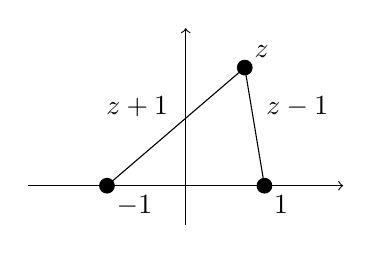
\begin{tikzpicture}
        \draw[->] (-2,0) -- (2,0);
        \draw[->] (0, -0.5) -- (0,2);

        \fill (1,0) circle (0.1);
        \fill (-1,0) circle (0.1);
        \fill (0.75,1.5) circle (0.1);

        \draw[below right] node at (-1,0) {$-1$};
        \draw[below right] node at (1,0) {$1$};
        \draw[above right] node at (0.75,1.5) {$z$};

        \draw (-1,0) -- (0.75,1.5);
        \draw (1,0) -- (0.75,1.5);
        
        \draw[above left] node at (-0.1,0.75) {$\abs{z+1}$};
        \draw[above right] node at (0.9,0.75) {$\abs{z-1}$};
        
        
    \end{tikzpicture}
\end{center}

And thus $f^{-1} (\Tilde{\om}) \subset D$.

Then with some calculation we find that, letting $z=x+iy$:
\begin{align*}
    \Im \br{f^{-1}(z)} = \frac{2y}{(x+1)^2 + y^2} > 0.
\end{align*}

Thus $f^{-1} (\Tilde{\om}) \subset \HH$. It follows that $f^{-1} (\Tilde{\om}) \subset \om$, thus $f$ has a well defined inverse and is thus bijective. Thus $f$ is biholomorphic. It follows that $F \circ f :\om \to D$ is a biholomorphism, so we are done.
\end{example}

\begin{example}[Infinite Strip]

Let $\om = \set{z \in \C \mid \Im(z) \in (0, \pi) }$.

\begin{center}
    \begin{tikzpicture}
        \begin{scope}
        \draw[->] (-2,0 ) -- (2,0);
        \draw[->] (0, -0.5) -- (0,2);

        \fill[pattern=north west lines] (-3,0) rectangle (3,1);
        \fill (0,1) circle (0.05);
        \draw[above right] node at (0,1) {$\pi i$};
        \fill (0,0) circle (0.05);
        \draw[below right] node at (0,0) {$0$};
        \draw node at (3.5,0.5) {$\Omega$};
        \end{scope}
    \end{tikzpicture}
\end{center}

Then $f: \om \to \HH, \, z \mapsto e^z$ is a biholomorphism with $f^{-1} : z \mapsto \log(z)$ as an inverse, where $\log$ is the branch on $\HH$ that takes $z$ to $\log(r) + i \theta$ with $ z = re^{i \theta}, \, \theta \in (0, \pi)$. Thus $\Im (\log(z)) \in (0, \pi)$ for $z \in \HH$. Thus $f^{-1} (\HH) \subset \om$.

Then, noting that $\sin(y) > 0$ for $y \in (0,\pi)$, $f(\om) \subset \HH$ since:
\begin{align*}
    \Im \br{e^z} &= \Im \br{e^x e^{iy}}\\
    &= \Im \br{e^x(\cos(y) + i \sin(y))}\\
    &= e^x \sin(y) > 0,
\end{align*}
thus the $\HH$ and $\om$ are biholomorphic, and thus we have found a biholomorphism between $\om$ and $D$.

\end{example}

We now move to a new topic -- the study of the Euler Gamma Function.

\section{Euler Gamma Function}

The Gamma function is usually studied in real analysis, but we will generalize it to $\C$. This leads to the Zeta function, which has many applications in fields such as number theory.

\begin{definition}[Positive Gamma Function]

Let $s \in (0,\infty) \subset \R$. Then we define the \textbf{positive gamma function} as:
\begin{align*}
    \Gamma(s) \defas \int_0^\infty e^{-t} t^{s-1} \dif t.
\end{align*}

\end{definition}

\begin{remark}
This integral is improper. To check for convergence we note that: 
\begin{itemize}
    \item Near $\infty$, the integrand $\leq C e^{\frac{-t}{2}}$ (since $e^{-t}$ shrinks fast), thus it converges at $\infty$.
    \item Near $0$,  the integrand $\leq t^{s-1}$ (which converges for $s>0$), thus it converges at $0$.
\end{itemize}
So this integral converges.

\end{remark}

\begin{note}
The bound of $C e^{\frac{-t}{2}}$ comes from the fact that $e^{-t} t^{s-1} = e^{-\frac{t}{2}} \cdot e^{-\frac{t}{2}} t^{s-1}$, and noting that for $t \in [1,\infty),$ $e^{-\frac{t}{2}} t^{s-1} < C$ for some $C \in \R$.
\end{note}


\begin{proposition}\label{prop:g-extension}
$\Gamma$ has an extension to a holomorphic function $\Gamma(s)$ defined on the half plane $\set{ s \in \C \mid \Re(s) > 0}$ given by the same formula where $t^{s-1} = e^{(s-1) \log(t)}$, with $\log(t)$ the usual natural log (since $0 < t < \infty$).
\end{proposition}

\begin{proof}
It suffices to show that $\Gamma(s) = \int_0^\infty e^{-t} t^{s-1} \dif t$ is a holomorphic function on $\set{ s \in \C \mid \Re(s) > 0}$, since it's obviously equal to the real equivalent (where the real version is defined).

Let $F_\varepsilon (s) \defas \int_\varepsilon^{1/\varepsilon} e^{-t} t^{s-1} \dif t  $. Then we are trying to define:
\begin{align*}
 \Gamma(s) = \lim_{\varepsilon \downarrow 0} F_\varepsilon (s) \defas \lim_{\varepsilon \downarrow 0} \int_\varepsilon^\frac{1}{\varepsilon} e^{-t} t^{s-1} \dif t .
\end{align*}

We firstly claim that $F_\varepsilon(s)$ is holomorphic in $\set{ s \in \C \mid \Re(s) > 0}$.


\begin{lemma}[General Fact]\label{lem:pos-gam-lem}
If $\oic$ open, $F(z,t)$ a continuous function on $\om \times [a,b]$ which for each $t \in [a,b]$ is such that $F(z,t)$ is holomorphic in $z \in \om$. Then $f(z) \defas \int_a^b F(z,t) \dif t$ is holomorphic in $\om$.

\end{lemma}


\begin{proof}[\ref{lem:pos-gam-lem}]
To prove this fact, it suffices to check that $\forall D \ssubset \om$, $f$ is holomorphic on $D$. By corollary (\ref{cor:morera}), it is enough to check that $\forall T \subset D$ triangle the integral over the boundary of the triangle is $0$. Then:
\begin{align*}
    \int_{\partial T} f(z) \dif z &= \int_{\partial T} \int_a^b F(z,t) \dif t \dif z\\
    \text{(Fubini) } &=  \int_a^b \br{ \int_{\partial T} F(z,t) \dif z } \dif t \\
    \text{(equation (\ref{eq:cauchy-int-fla})) } &= \int_a^b \br{0} \dif t = 0.
\end{align*}
And we are done.
\end{proof}

To apply this lemma, let $\om = \set{ s \in \C \mid \Re(s) > 0}$, $[a,b] = [\varepsilon, \frac{1}{\varepsilon} ]$, $F(z,t) = e^{-t} t^{z-1} $. Then $F_\varepsilon$ is holomorphic on $\om$. Fix any $M > \delta >0$. Then consider:
\begin{align*}
    \om_{\delta, M} \defas \set{s \in \C \mid \delta < \Re(s) < M}.
\end{align*}

\begin{center}
    \begin{tikzpicture}
        \draw[->] (-0.5,0) -- (3,0);
        \draw[->] (0, -2) -- (0,2);
        \fill[pattern=north west lines] (1,-3) rectangle (2,3);
        \draw[above left] node at (1,0) {$\delta$};
        \draw[above right] node at (2,0) {$M$};
        \fill (1,0) circle (0.05);
        \fill (2,0) circle (0.05);
    \end{tikzpicture}
\end{center}


Note that for $\sigma = \Re (s)$ we have:
\begin{align*}
    \abs{e^{-t}t^{s-1}} = \abs{e^{-t}e^{(s-1) \log(t)}} = \abs{e^{-t}e^{(\sigma-1) \log(t)}} = e^{-t}t^{\sigma-1}.
\end{align*}

Then on this strip (ie points $s$ such that $\delta < \sigma < M$) we can estimate:
\begin{align*}
    \abs{\Gamma(s) - F_\varepsilon(s)} &= \abs{\int_0^\varepsilon e^{-t} t^{s-1} \dif t + \int_\frac{1}{\varepsilon}^\infty e^{-t} t^{s-1} \dif t}\\
    & \leq \int_0^\varepsilon e^{-t} t^{\sigma-1} \dif t + \int_\frac{1}{\varepsilon}^\infty e^{-t} t^{\sigma-1} \dif t.
\end{align*}

Noting that:
\begin{align*}
    \int_0^\varepsilon e^{-t} t^{\sigma-1} \dif t \leq \int_0^\varepsilon t^{\sigma-1} \dif t = \frac{\varepsilon^\sigma}{\sigma} \leq \frac{\varepsilon^\delta}{\delta} \xrightarrow[]{\varepsilon \to 0} 0.
\end{align*}

And that:
\begin{align*}
    \int_\frac{1}{\varepsilon}^\infty e^{-t} t^{\sigma-1} \dif t &\leq \int_\frac{1}{\varepsilon}^\infty e^{-t} t^{M-1} \dif t\\
    \text{($t\in [\tfrac{1}{\varepsilon}, \infty)$) } &\leq \int_\frac{1}{\varepsilon}^\infty C_M e^{-\frac{t}{2}} \dif t\\
    &= C_M \br{-2 e^{\frac{-t}{2}}} \bigg|_\frac{1}{\varepsilon}^\infty\\
    &= 2C_M e^{\frac{-1}{2\varepsilon}} \xrightarrow[]{\varepsilon \to 0} 0.
\end{align*}

We have that for all $s$:
\begin{align*}
    \abs{\Gamma(s) - F_\varepsilon(s)} = 0.
\end{align*}

It follows that $F_\varepsilon \tou \Gamma$ on $\om_{\delta, M}$, and thus that $\Gamma $ is holomorphic on $\om_{\delta, M}$. It follows that $\Gamma$ is holomorphic on $\om$.
\end{proof}


